\documentclass[12pt]{beamer}
\usepackage[UTF8]{ctex}
\usepackage{graphicx}
\usepackage{amsmath}
\usepackage{booktabs}
\usepackage{multirow}
\usepackage{xcolor}
\usepackage{listings}
\usepackage{tikz}
\usetikzlibrary{shapes.geometric}
\usepackage{pgfplots}
\pgfplotsset{compat=1.18}

% 主题设置
\usetheme{Madrid}
\usecolortheme{default}

% 标题信息
\title{基于深度学习的植物纤维图像分类系统}
\subtitle{阶段性进展汇报 - ResNet-50迁移学习初步探索}
\author{项目汇报}
\institute{植物纤维识别项目组}
\date{\today}

% 自定义颜色
\definecolor{darkblue}{RGB}{0,51,102}
\definecolor{lightblue}{RGB}{173,216,230}
\definecolor{darkgreen}{RGB}{0,100,0}

\begin{document}

% 标题页
\frame{\titlepage}

% 目录
\begin{frame}
\frametitle{汇报大纲}
\tableofcontents
\end{frame}

% 第一部分:项目概述
\section{项目概述}

\begin{frame}
\frametitle{项目背景与目标}
\begin{itemize}
    \item \textbf{研究背景}:植物纤维识别在材料科学、生物学研究中具有重要意义
    \item \textbf{项目目标}:探索基于深度学习的植物纤维自动分类可行性
    \item \textbf{技术路线}:采用ResNet-50预训练模型进行迁移学习
    \item \textbf{当前阶段}:初步验证技术方案,识别关键挑战
\end{itemize}

\vspace{0.3cm}
\begin{block}{探索重点}
\begin{itemize}
    \item 多模态图像融合(光镜+电镜)
    \item 小样本数据集的处理策略
    \item 类别不平衡问题的解决方案
\end{itemize}
\end{block}
\end{frame}

\begin{frame}
\frametitle{数据集概况}
\begin{columns}
\begin{column}{0.5\textwidth}
\textbf{数据集统计:}
\begin{itemize}
    \item 总图像数量:\textcolor{darkblue}{295张}
    \item 光镜图像:147张 (49.8\%)
    \item 电镜图像:148张 (50.2\%)
    \item 植物类别:6种
\end{itemize}

\vspace{0.3cm}
\textbf{图像特征:}
\begin{itemize}
    \item 主要尺寸:1600×1200像素
    \item 文件格式:TIFF、PNG
    \item 平均大小:3.78MB
\end{itemize}
\end{column}

\begin{column}{0.5\textwidth}
\textbf{类别分布:}
\begin{table}[h]
\centering
\small
\begin{tabular}{lc}
\toprule
\textbf{植物类别} & \textbf{图像数量} \\
\midrule
粽叶芦 & 65 \\
怀槐 & 54 \\
硬头黄 & 52 \\
长叶水麻 & 49 \\
鼠皮树 & 42 \\
蒙古栎 & 33 \\
\bottomrule
\end{tabular}
\end{table}
\end{column}
\end{columns}
\end{frame}

% 第二部分:技术方案
\section{技术方案}

\begin{frame}
\frametitle{系统架构设计}
\begin{center}
\begin{tikzpicture}[node distance=2cm, auto,
    process/.style={rectangle, minimum width=2.5cm, minimum height=1cm, text centered, draw=black, fill=lightblue},
    data/.style={ellipse, minimum width=2cm, minimum height=0.8cm, text centered, draw=black, fill=yellow!30},
    arrow/.style={thick,->,>=stealth}]
    
    % 节点定义
    \node [data] (input) {原始图像};
    \node [process, below of=input] (preprocess) {数据预处理};
    \node [process, below of=preprocess] (augment) {数据增强};
    \node [process, below of=augment] (model) {ResNet-50模型};
    \node [data, below of=model] (output) {分类结果};
    
    % 连接线
    \draw [arrow] (input) -- (preprocess);
    \draw [arrow] (preprocess) -- (augment);
    \draw [arrow] (augment) -- (model);
    \draw [arrow] (model) -- (output);
    
    % 侧边注释
    \node [right of=preprocess, node distance=3cm] {尺寸调整、标准化};
    \node [right of=augment, node distance=3cm] {翻转、旋转、颜色变换};
    \node [right of=model, node distance=3cm] {迁移学习、微调};
\end{tikzpicture}
\end{center}
\end{frame}

\begin{frame}
\frametitle{ResNet-50模型架构}
\begin{columns}
\begin{column}{0.6\textwidth}
\textbf{网络结构:}
\begin{itemize}
    \item \textbf{骨干网络}:ResNet-50 (ImageNet预训练)
    \item \textbf{特征提取}:2048维特征向量
    \item \textbf{分类头}:全连接层 + Dropout
    \item \textbf{输出层}:6类softmax分类
\end{itemize}

\vspace{0.3cm}
\textbf{迁移学习策略:}
\begin{itemize}
    \item 冻结前期卷积层参数
    \item 微调后期特征层
    \item 重新训练分类头
\end{itemize}
\end{column}

\begin{column}{0.4\textwidth}
\begin{block}{模型参数}
\small
\begin{itemize}
    \item 输入尺寸:224×224×3
    \item 批次大小:32
    \item 学习率:0.001
    \item 优化器:Adam
    \item 训练轮数:50
    \item 权重衰减:1e-4
\end{itemize}
\end{block}
\end{column}
\end{columns}
\end{frame}

\begin{frame}
\frametitle{ResNet-50理论基础}
\textbf{为什么选择ResNet-50?}
\begin{itemize}
    \item 传统深度网络存在"梯度消失"问题:信息在反向传播时逐层衰减
    \item ResNet通过"跳跃连接"让信息可以直接传递到后面的层
    \item 就像给信息建了一条"高速公路",避免拥堵
\end{itemize}

\vspace{0.2cm}
\textbf{残差块的核心思想:}
\[
\mathbf{y} = \mathcal{F}(\mathbf{x}, \{W_i\}) + \mathbf{x}
\]
\small{输出 = 学到的变化 + 原始输入(这样即使学不到什么,至少能保持原样)}

\vspace{0.2cm}
\textbf{Bottleneck结构(降低计算量):}
\[
\begin{aligned}
\text{1×1卷积} &\rightarrow \text{降维(减少通道数)} \\
\text{3×3卷积} &\rightarrow \text{特征提取(核心计算)} \\
\text{1×1卷积} &\rightarrow \text{升维(恢复通道数)}
\end{aligned}
\]
\end{frame}

\begin{frame}
\frametitle{损失函数与优化策略}
\textbf{如何衡量模型的"错误程度"?}
\begin{itemize}
    \item 使用交叉熵损失:预测越准确,损失越小
    \item 当模型完全猜对时,损失为0;完全猜错时,损失很大
\end{itemize}

\textbf{交叉熵损失函数:}
\[
\mathcal{L} = -\frac{1}{N}\sum_{i=1}^{N}\sum_{j=1}^{C} y_{ij} \log(\hat{y}_{ij})
\]
\small{\(N\)=样本数量,\(C\)=类别数量,\(y_{ij}\)=真实标签,\(\hat{y}_{ij}\)=预测概率}

\textbf{Softmax:将输出转换为概率}
\[
\hat{y}_{ij} = \frac{\exp(z_{ij})}{\sum_{k=1}^{C} \exp(z_{ik})}
\]
\small{确保所有类别的预测概率加起来等于1}

\textbf{Adam优化器:智能调整学习步长}
\[
\theta_{t+1} = \theta_t - \frac{\alpha}{\sqrt{\hat{\mathbf{v}}_t} + \epsilon} \hat{\mathbf{m}}_t
\]
\small{结合了动量和自适应学习率,训练更稳定}
\end{frame}

\begin{frame}
\frametitle{数据处理策略}
\begin{columns}
\begin{column}{0.5\textwidth}
\textbf{数据预处理:}
\begin{itemize}
    \item 图像尺寸标准化:224×224
    \item RGB格式转换
    \item ImageNet标准化
    \item 多格式支持(TIFF/PNG/JPG)
\end{itemize}

\vspace{0.3cm}
\textbf{数据增强:}
\begin{itemize}
    \item 随机水平/垂直翻转
    \item 随机旋转(±30°)
    \item 颜色抖动变换
    \item 随机裁剪
\end{itemize}
\end{column}

\begin{column}{0.5\textwidth}
\textbf{数据集划分:}
\begin{itemize}
    \item 训练集:70\%
    \item 验证集:15\%
    \item 测试集:15\%
    \item 分层采样保证类别平衡
\end{itemize}

\vspace{0.3cm}
\textbf{不平衡处理:}
\begin{itemize}
    \item 加权随机采样
    \item 类别权重调整
    \item 数据增强补偿
\end{itemize}
\end{column}
\end{columns}
\end{frame}

% 第三部分:实验结果
\section{实验结果}

\begin{frame}
\frametitle{训练过程监控}
\begin{columns}
\begin{column}{0.5\textwidth}
\begin{figure}
\centering
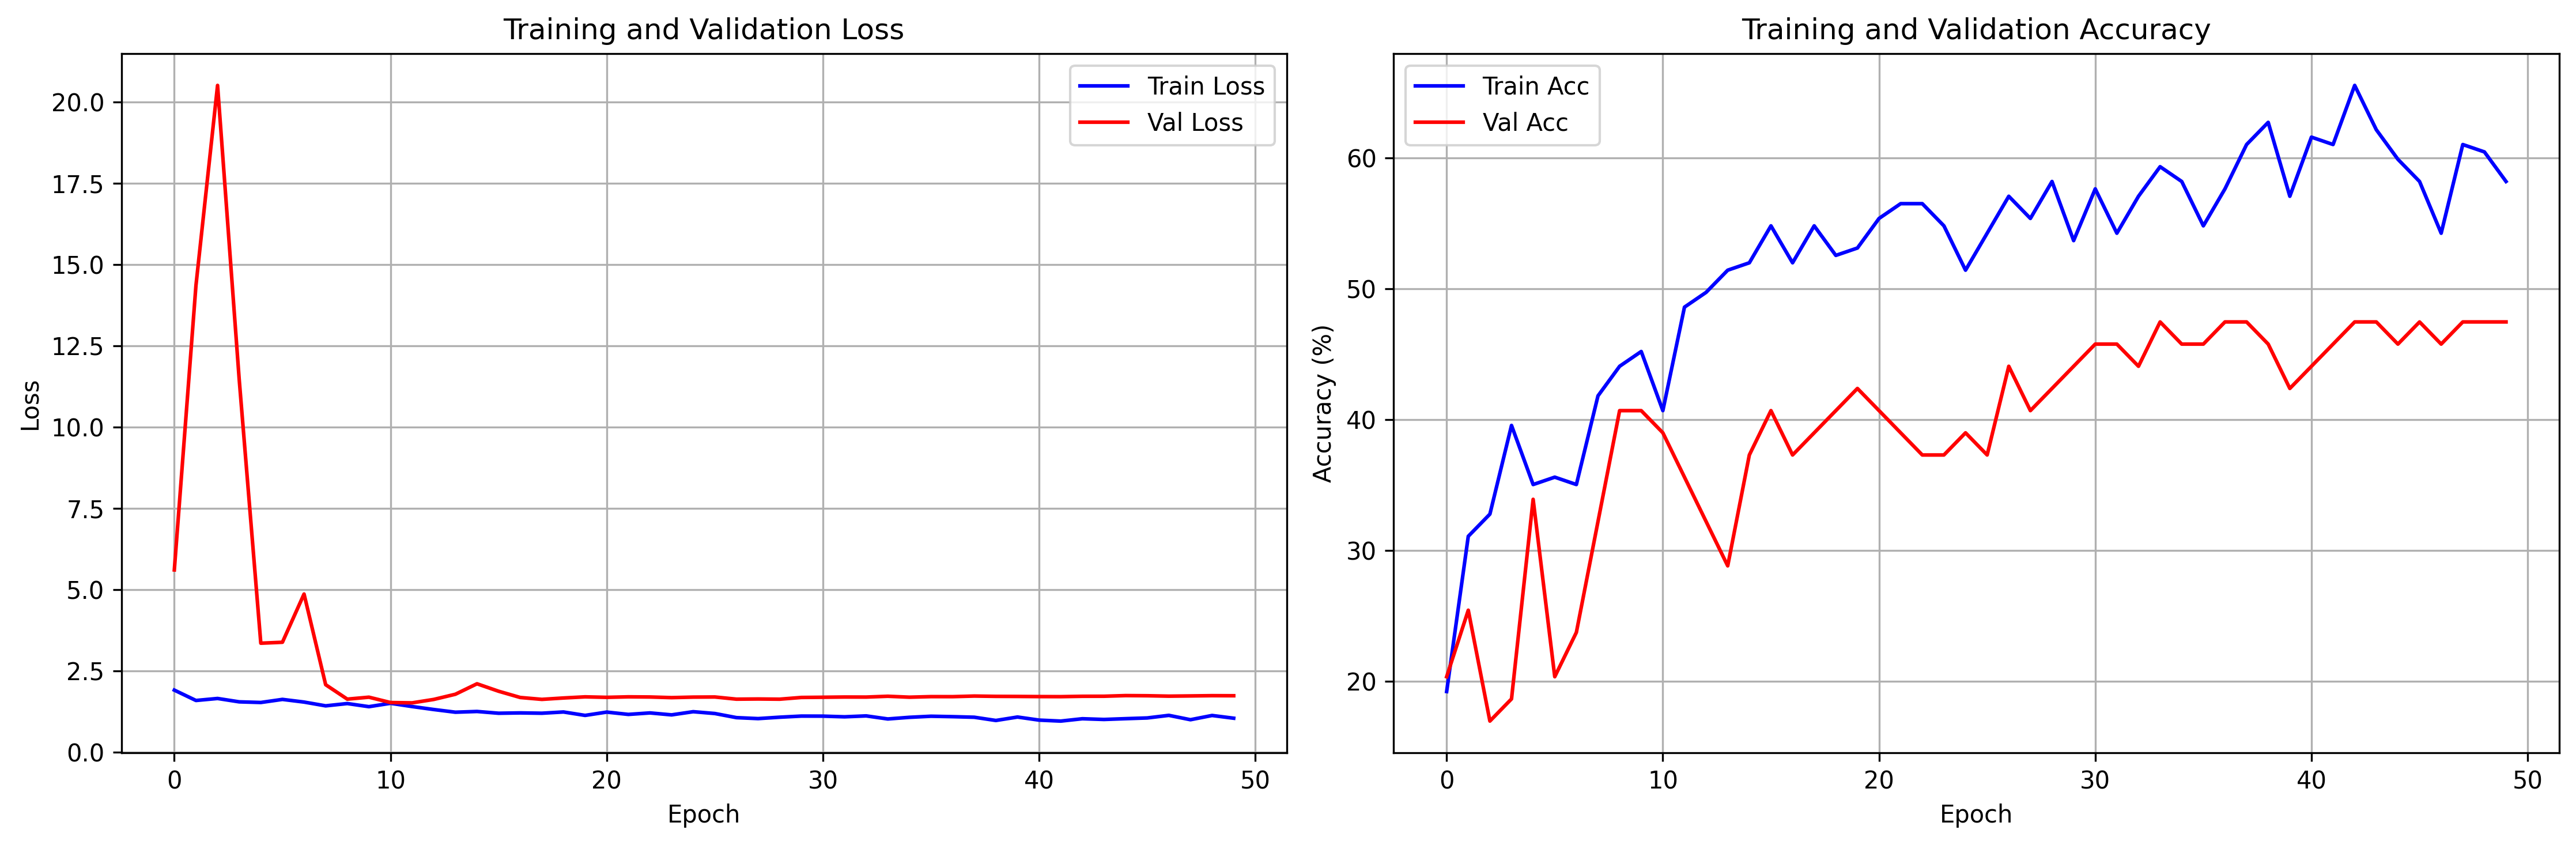
\includegraphics[width=\textwidth]{training_history.png}
\caption{训练历史曲线}
\end{figure}
\end{column}

\begin{column}{0.5\textwidth}
\textbf{训练观察:}
\begin{itemize}
    \item 训练损失下降较快
    \item 验证准确率提升有限
    \item 存在训练验证差距
    \item 收敛到局部最优
\end{itemize}

\vspace{0.3cm}
\begin{block}{关键指标}
\begin{itemize}
    \item 最佳验证准确率:\textcolor{darkgreen}{47.46\%}
    \item 测试集准确率:\textcolor{darkgreen}{44.07\%}
    \item 训练时间:约33分钟
\end{itemize}
\end{block}
\end{column}
\end{columns}
\end{frame}

\begin{frame}
\frametitle{分类性能评估}
\begin{columns}
\begin{column}{0.5\textwidth}
\begin{figure}
\centering
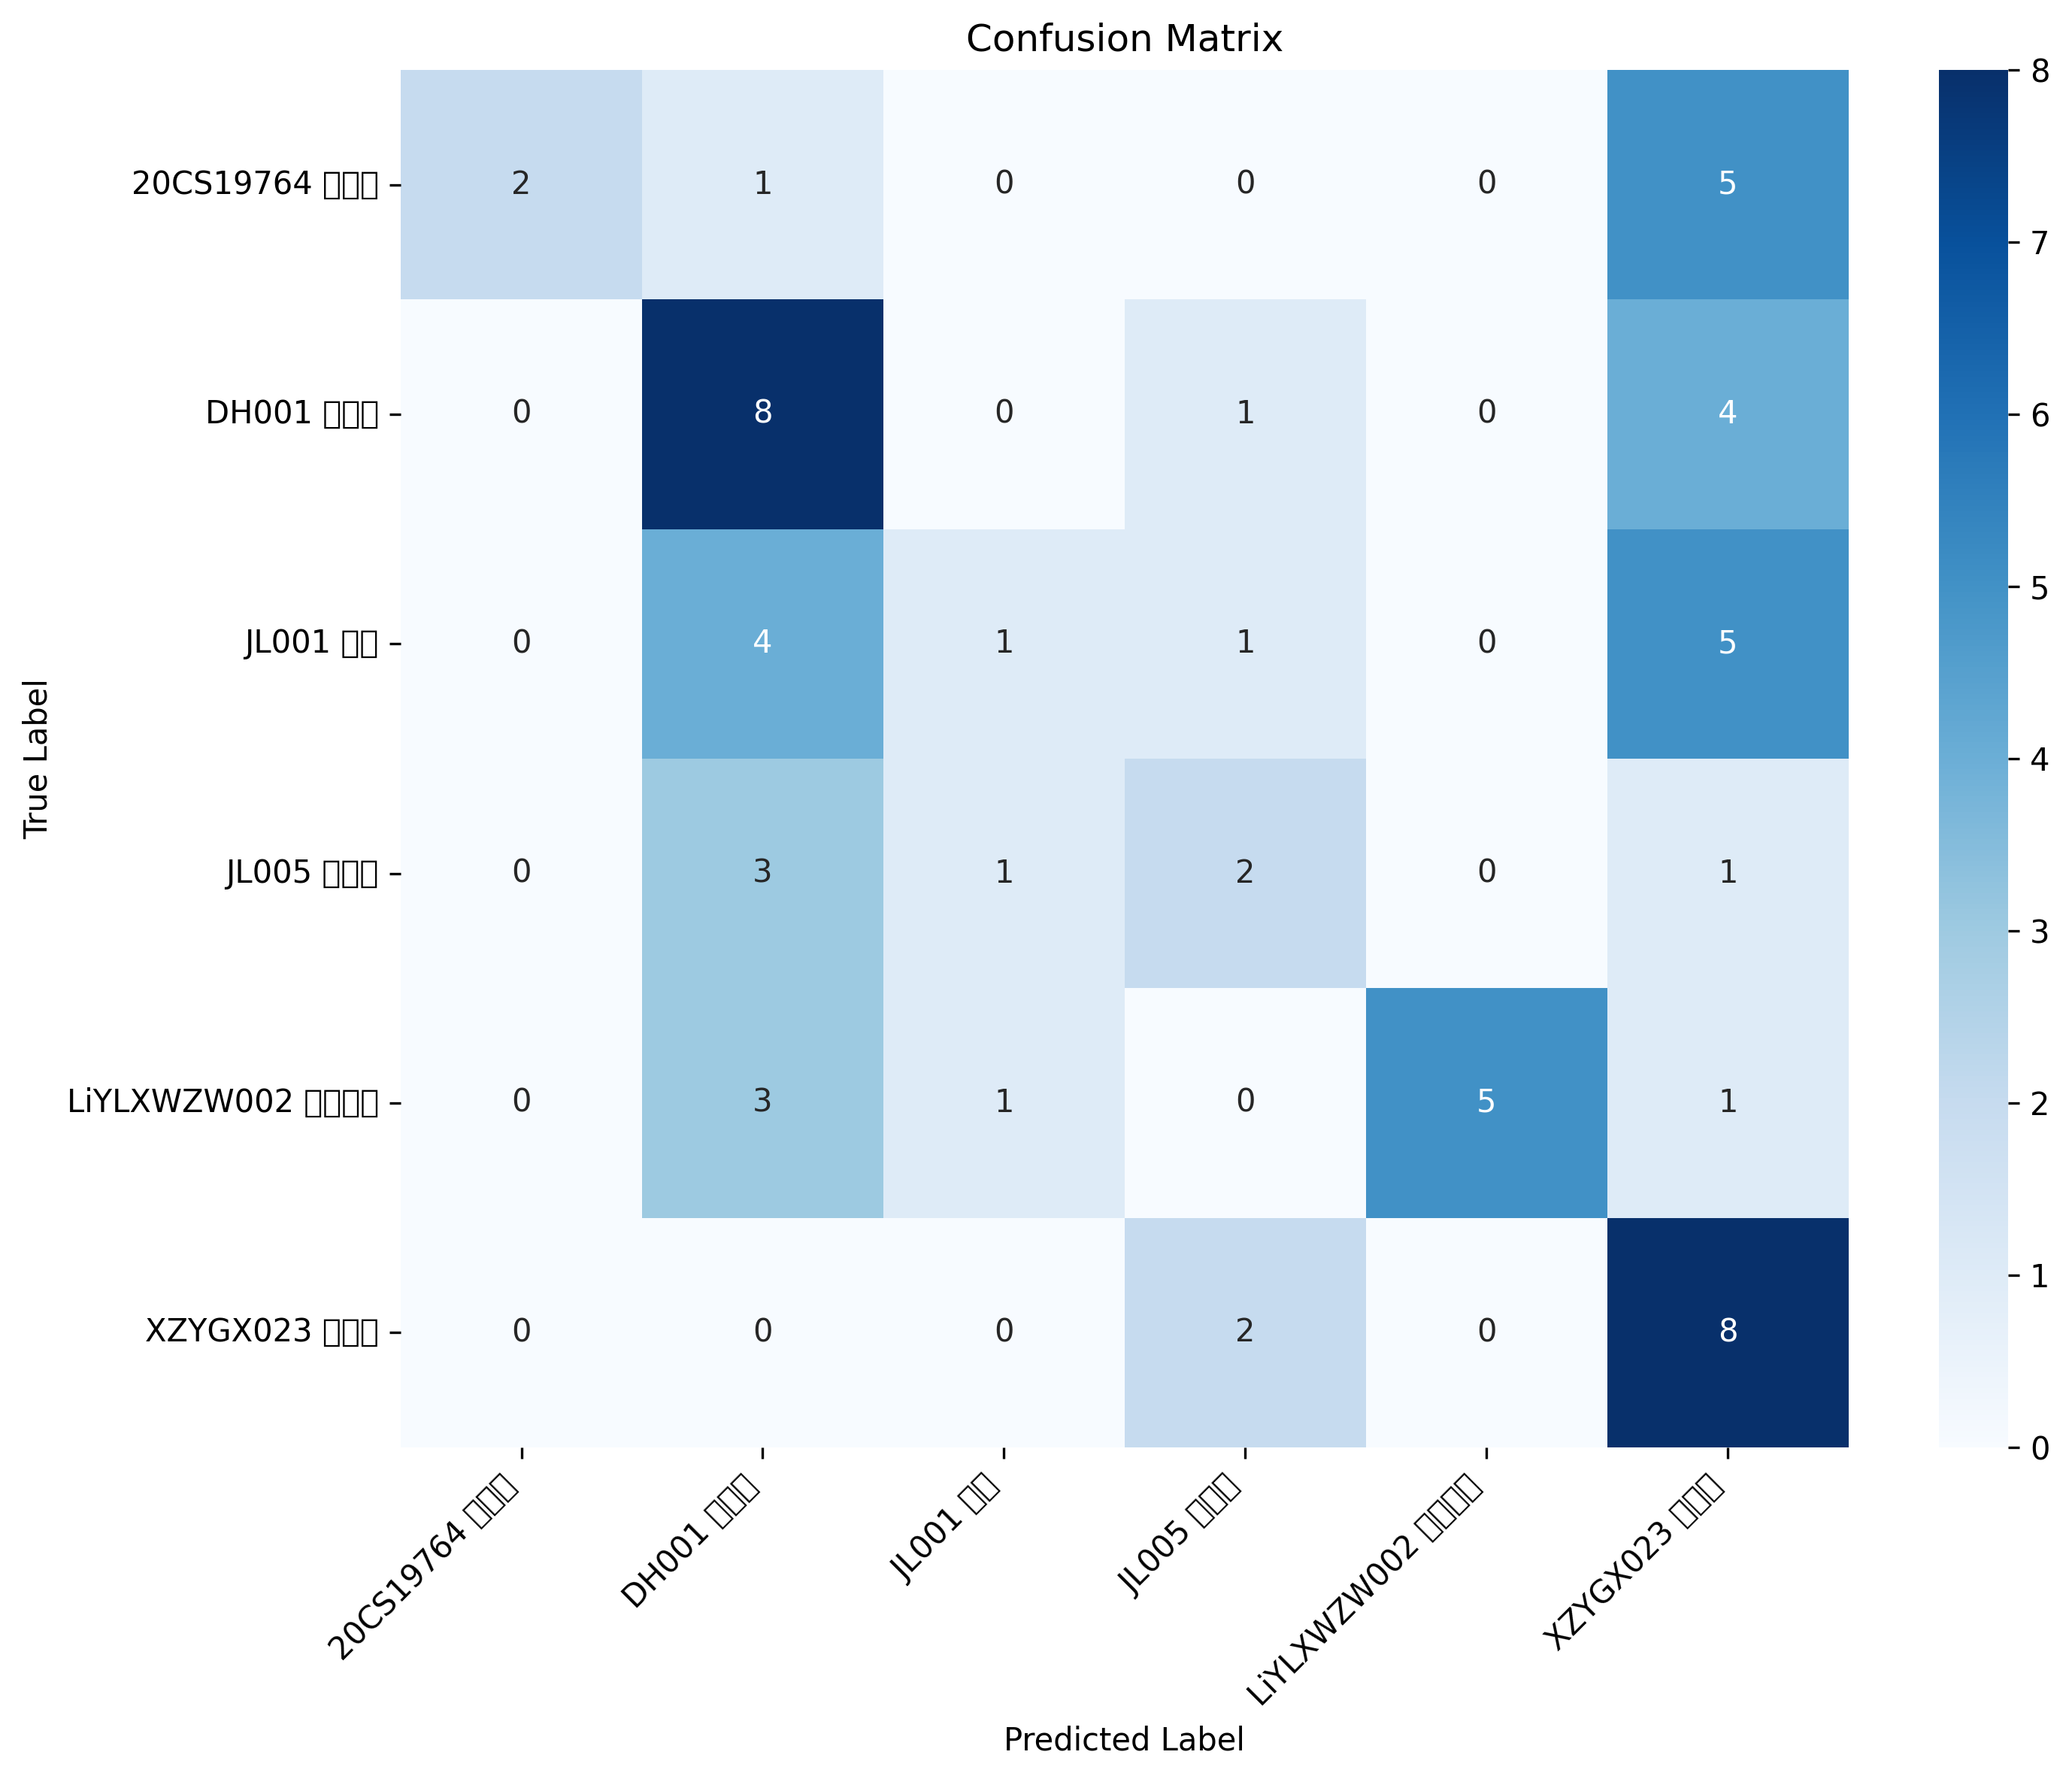
\includegraphics[width=\textwidth]{confusion_matrix.png}
\caption{混淆矩阵}
\end{figure}
\end{column}

\begin{column}{0.5\textwidth}
\textbf{性能分析(存在明显问题):}
\begin{itemize}
    \item 整体准确率偏低(44.07\%),远未达到实用标准
    \item 各类别表现差异很大,模型学习不充分
    \item 数据量不足是主要瓶颈(仅295张图像)
    \item 类别不平衡加剧了分类困难
\end{itemize}

\vspace{0.3cm}
\begin{block}{评估指标}
\small
\begin{itemize}
    \item 宏平均精确率:57\%
    \item 宏平均召回率:42\%
    \item 宏平均F1分数:41\%
    \item 加权平均准确率:44.07\%
\end{itemize}
\end{block}
\end{column}
\end{columns}
\end{frame}

\begin{frame}
\frametitle{数据集分析可视化}
\begin{figure}
\centering
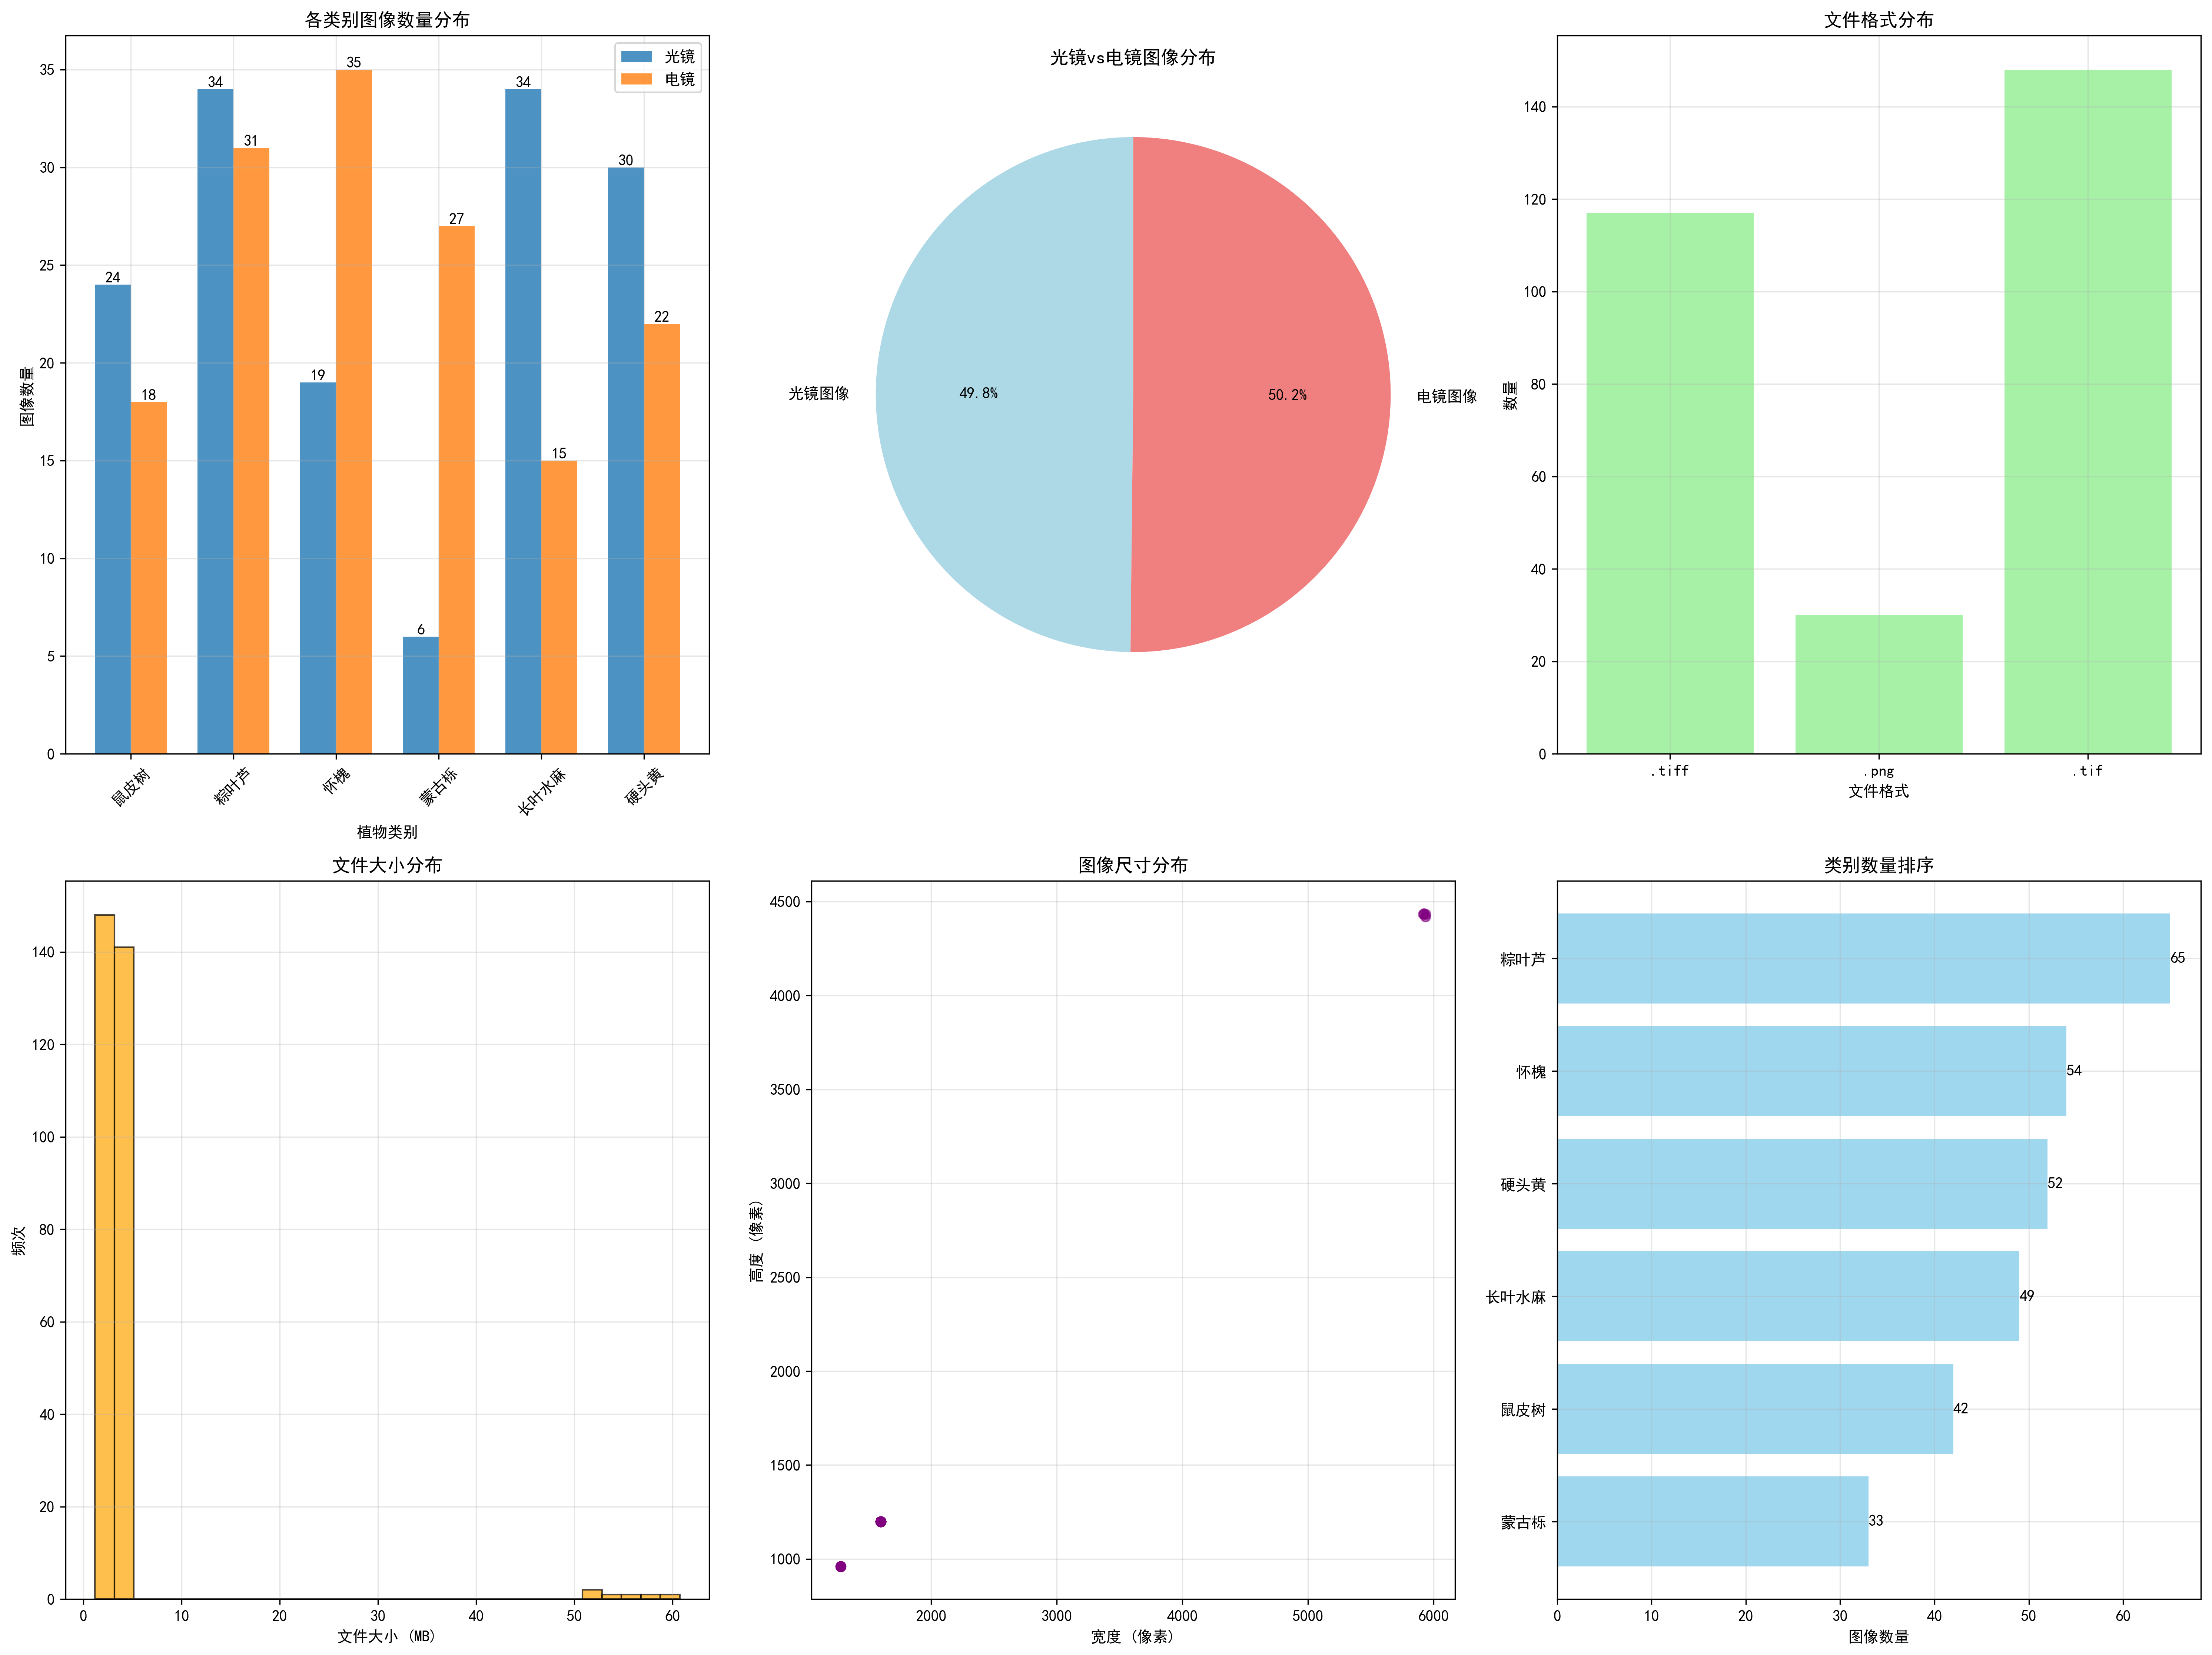
\includegraphics[width=0.8\textwidth]{dataset_analysis.png}
\caption{数据集统计分析图表}
\end{figure}

\begin{itemize}
    \item 类别分布相对均衡,但存在一定不平衡
    \item 光镜与电镜图像数量基本相等
    \item 图像尺寸较为统一,有利于模型训练
\end{itemize}
\end{frame}

% 第四部分:项目成果
\section{项目成果}

\begin{frame}
\frametitle{项目交付物}
\begin{columns}
\begin{column}{0.5\textwidth}
\textbf{核心代码模块:}
\begin{itemize}
    \item \texttt{train.py} - 模型训练脚本
    \item \texttt{predict.py} - 预测推理脚本
    \item \texttt{analyze\_dataset.py} - 数据分析工具
\end{itemize}

\vspace{0.3cm}
\textbf{配置文件:}
\begin{itemize}
    \item \texttt{config.json} - 训练参数配置
    \item \texttt{requirements.txt} - 依赖包列表
    \item \texttt{.gitignore} - 版本控制配置
\end{itemize}
\end{column}

\begin{column}{0.5\textwidth}
\textbf{模型文件:}
\begin{itemize}
    \item 训练好的ResNet-50模型
    \item 模型权重和配置信息
    \item 类别映射关系
\end{itemize}

\vspace{0.3cm}
\textbf{分析报告:}
\begin{itemize}
    \item 数据集统计报告(JSON)
    \item 训练历史可视化
    \item 混淆矩阵分析
    \item 性能评估报告
\end{itemize}
\end{column}
\end{columns}
\end{frame}

\begin{frame}
\frametitle{技术特色与创新}
\begin{block}{技术亮点}
\begin{itemize}
    \item \textbf{多模态融合}:统一处理光镜和电镜图像,提升模型泛化能力
    \item \textbf{迁移学习}:充分利用ImageNet预训练权重,加速收敛
    \item \textbf{数据增强}:丰富的增强策略,提高模型鲁棒性
    \item \textbf{不平衡处理}:加权采样策略,解决类别不均衡问题
\end{itemize}
\end{block}

\begin{block}{工程实践}
\begin{itemize}
    \item \textbf{模块化设计}:代码结构清晰,易于维护和扩展
    \item \textbf{完整文档}:详细的README和代码注释
    \item \textbf{可视化分析}:丰富的图表和统计信息
    \item \textbf{自动化流程}:一键训练和预测功能
\end{itemize}
\end{block}
\end{frame}

% 第五部分:总结与展望
\section{总结与展望}

\begin{frame}
\frametitle{项目总结}
\begin{block}{已完成工作}
\begin{itemize}
    \item ✅ 完成数据集收集和预处理
    \item ✅ 实现基于ResNet-50的分类模型
    \item ✅ 完成模型训练和性能评估
    \item ✅ 开发预测和分析工具
    \item ✅ 生成完整的项目文档
\end{itemize}
\end{block}

\begin{block}{阶段性成果}
\begin{itemize}
    \item 完成了技术方案的初步验证
    \item 识别了数据不足等关键瓶颈
    \item 建立了基础的分类流水线
    \item 为后续改进提供了基准
\end{itemize}
\end{block}

\begin{alertblock}{当前挑战}
\begin{itemize}
    \item 准确率44.07\%距离实用化还有很大差距
    \item 数据集规模严重不足
    \item 类别不平衡问题突出
\end{itemize}
\end{alertblock}
\end{frame}

\begin{frame}
\frametitle{下一步改进计划}
\begin{block}{\textbf{紧急优先级 - 数据问题}}
\begin{itemize}
    \item \textbf{扩大数据集}:目标收集至少1000张图像
    \item \textbf{平衡类别分布}:确保每类至少100张样本
    \item \textbf{提高数据质量}:标注一致性检查
\end{itemize}
\end{block}

\begin{block}{\textbf{中期目标 - 技术优化}}
\begin{itemize}
    \item 尝试更适合小样本的网络架构
    \item 改进数据增强策略
    \item 探索半监督学习方法
    \item 引入领域自适应技术
\end{itemize}
\end{block}

\begin{block}{\textbf{长期规划 - 系统完善}}
\begin{itemize}
    \item 达到80\%以上的实用准确率
    \item 开发用户友好的应用界面
    \item 建立持续学习机制
\end{itemize}
\end{block}
\end{frame}



\end{document}